%!TEX root = ../Thesis.tex

\section{Feed forward Neural Network}
\label{sec:theory:ffnn}

The models presented in this thesis are all neural networks or can be interpreted as such. To give a short introduction to neural networks in general the feed forward neural network (FFNN) is used. The feed forward neural network is one of the simplest models in the family of neural networks. The other models used in this thesis can be considered as extensions of the FFNN. An exception to this is perhaps the skip-gram model which is a simplified version of FFNN.

\subsection{The neuron}

The neuron is the main construct in any neural network. Mathematically it is just a function which takes a vector and returns a scalar. It does this by a weighted sum of the inputs $\{ x_i \}_{i=1}^I$:
\begin{equation}
a = \sum_{i=1}^I w_{i} x_i
\end{equation}

This sum is then typically transformed using a non-linear function $\theta$:
\begin{equation}
b = \theta(a)
\end{equation}

The value $b$ is the output of the neuron and is called the \textit{activation}. Typically the sigmoid function $\sigma(\cdot)$ or hyperbolic tangent $\tanh(\cdot)$ function is used as non-linear function $\theta$ \cite{bishop}. If no non-linear function is applied then the identity function is used, $\theta(a) = a$.

\begin{figure}[H]
	\centering
	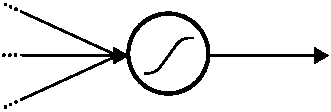
\includegraphics[scale=0.7]{theory/ffnn-neuron}
	\caption{Visual representation of a single neuron. The left arrows represents the input elements $\{ x_i \}_{i=1}^I$. The circle represent the function that returns the scalar $b$ (right arrow).}
\end{figure}

\subsection{The network}

A neural network is a multivariate non-linear regression model constructed by combining neurons, but the network can be slightly expanded to become a multiclass classifier. This is done by using the softmax function \cite{the-elements-of-statistical-learning}, such each output value is the class probability $y_k = P(C_k | x)$.

\begin{figure}[h]
	\centering
	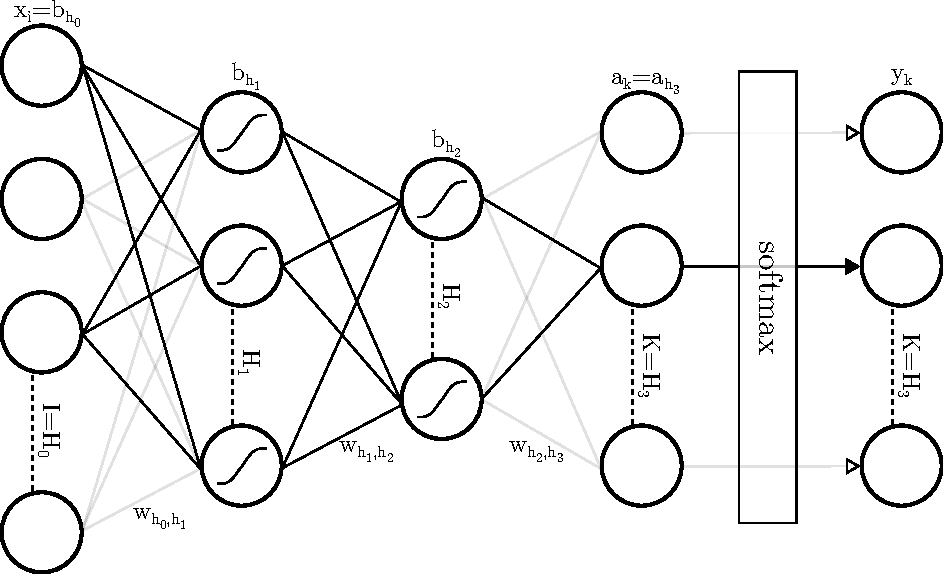
\includegraphics[scale=0.7]{theory/ffnn-network.pdf}
	\caption{Visual representation of a neural network with two hidden layers. Some lines are less visible, this is just a visual aid because the many lines can be difficult to look at.}
	\label{fig:theory:ffnn:network}
\end{figure}

The neural network in Figure \ref{fig:theory:ffnn:network}, have one input layer $x_i, i \in [1, I]$ and one output layer $y_k, k \in [1, K]$. This is the same for any neural network, what varies is the type of network (here a feed forward neural network) and the amount of hidden layers (here two). The hidden layers are those layers there can contain non-linear functions. If there are no hidden layers, the neural network i just a multivariate linear regressor or a multiclass logistic regressor if the softmax is applied \cite{bishop}.

Because there are more than one neuron in each layer and many layers, the neuron index and layer index is denoted by the subscript. For example a neuron output is denoted by $b_{h_{\ell}}$ for $h_{\ell} \in [1, H_{\ell}]$, where $h_{\ell}$ is the neuron index and $H_\ell$ is the amount of neurons in layer $\ell$.

\subsection{Forward pass}

Calculation of the network output ($y_k$) is sometimes called the \textit{forward pass}, while the parameter estimation is sometimes called the \textit{backward pass}.

First the activation for the first layer is calculated:
\begin{equation}
\begin{aligned}
b_{h_1} = \theta(a_{h_1}), && a_{h_1} = \sum_{i = 1}^I w_{i, h_1} x_i, && \forall h_1 \in [1, H_1]
\end{aligned}
\end{equation}

The activation for the second layer is almost identical:
\begin{equation}
\begin{aligned}
b_{h_2} = \theta(a_{h_2}), && a_{h_2} = \sum_{h_1 = 1}^{H_1} w_{h_1, h_2} b_{h_1}, && \forall h_2 \in [1, H_2]
\end{aligned}
\end{equation}

In fact by letting $x_i = b_{h_0}$ the activation can be generalized to any amount of hidden layers ($L$):
\begin{equation}
\begin{aligned}
b_{h_\ell} &= \theta(a_{h_\ell}), && \forall h_{\ell} \in [1, H_{\ell}] \wedge \ell \in [1, L] \\
a_{h_\ell} &= \sum_{h_{\ell-1} = 1}^{H_{\ell-1}} w_{h_{\ell-1}, h_{\ell}} b_{h_{\ell-1}}, && \forall \ell \in [1, L+1] \text{ where: } b_{h_0} = x_i, H_0 = I \\
\end{aligned}
\end{equation}

Note that the last layer $\ell = L + 1$ does not use the non-linear $\theta$ function. 
At last the network output $y_k$ can be calculated using the softmax function on the $a_k = a_{L+1}$ values:
\begin{equation}
\begin{aligned}
y_k = \frac{\exp(a_k)}{\sum_{k'=1}^K \exp(a_{k'})}, && \forall k \in [1, K] \text{ where: } a_k=a_{h_{L+1}}, K = H_{L + 1}
\end{aligned}
\label{eq:theory:ffnn:y}
\end{equation}

\subsection{Loss function}

Optimization of the parameters $w_{i,j}$ requires definition of a loss function. For classification it makes sense to maximize the joint probability of observing all the observations:
\begin{equation}
P(\mathbf{t} | \mathbf{x}, \mathbf{w}) = \prod_{n=1}^N P(\mathbf{t}_n | \mathbf{x}_n, \mathbf{w})  = \prod_{n=1}^N \prod_{k=1}^K P(C_{n, k} | \mathbf{x}_n, \mathbf{w})^{t_{n, k}}
\end{equation}

Here $\mathbf{x}_{n}$ is the input vector for observation $n$, with a corresponding label vector $\mathbf{t}_n$. The label vector is an indicator vector, constructed using 1-of-K encoding. For example if there are 5 classes and class 2 is the correct class for observation $n$, then $\mathbf{t}_n = [0, 1, 0, 0, 0]^T$. The class probability $P(C_{n, k} | \mathbf{x}_n, \mathbf{w})$ is in terms of the forward pass equations the $y_k$ value for observation $n$.

The logarithm is then used to create linearity and avoid numerical floating point issues. The sign is also changed such that it becomes a loss function:
\begin{equation}
- \ln\left(P(\mathbf{t} | \mathbf{x}, \mathbf{w})\right) = - \sum_{n=1}^N \sum_{k=1}^K t_{n, k} \ln\left( P(C_{n, k} | \mathbf{x}_n, \mathbf{w})\right)
\label{eq:theory:ffnn:long-loss}
\end{equation}

Because of the linearity in \eqref{eq:theory:ffnn:long-loss} it makes sense to just consider the loss function for one datapoint. This way the $n$ index can be omitted from the equations and the sum over $n$ can always be reintroduced in the end. By doing this one gets the final loss function there will be denoted by $\mathcal{L}$:
\begin{equation}
\mathcal{L} = - \sum_{k=1}^K t_{k} \ln\left( P(C_{k} | \mathbf{x}, \mathbf{w})\right) =  - \sum_{k=1}^K t_k \ln(y_k)
\label{eq:theory:ffnn:loss}
\end{equation}

\subsection{Backward pass}

For the neural network there is no closed form solution to optimizing the loss function. Instead an iterative algorithm called \textit{gradient descent} is used. Gradient descent uses the derivatives of the loss function with respect to the parameters to iteratively optimize the parameters. This approach will be discussed in details later, for now the important part is to find a method of calculating the derivatives.

For calculating the derivatives the \textit{error backpropagation} algorithm is used. The name varies a bit depending on the neural network architecture, thus the term \textit{backward pass} will be used as the umbrella term.

The neural network from earlier in Figure \ref{fig:theory:ffnn:network} will be used to inspire the general algorithm. The overall goal is to calculate:
\begin{equation}
\begin{aligned}
\frac{\partial \mathcal{L}}{\partial w_{h_{\ell-1}, h_\ell}}, && \forall \ell \in [1, L + 1]
\end{aligned}
\label{eq:theory:ffnn:bprop-problem}
\end{equation} 

First consider the problem in \eqref{eq:theory:ffnn:bprop-problem} for the layer $\ell = 1$. The loss function depends on some hidden input from the first hidden layer $a_{h_1}$, thus the chain rule can be used:
\begin{equation}
\frac{\partial \mathcal{L}}{\partial w_{h_0, h_1}} = \frac{\partial \mathcal{L}}{\partial a_{h_1}} \frac{\partial a_{h_1}}{\partial w_{h_0, h_1}} =  \frac{\partial \mathcal{L}}{\partial a_{h_1}} x_{h_0}
\label{eq:theory:ffnn:bprop-firstlayer}
\end{equation}

It turns out that it is smart to define $\frac{\partial \mathcal{L}}{a_{h_1}}$ in general for all layers, this is just for bookkeeping, there makes it easier to implement.
\begin{equation}
\delta_{h_\ell} \defeq \frac{\partial \mathcal{L}}{\partial a_{h_\ell}}
\end{equation}

Using this \eqref{eq:theory:ffnn:bprop-firstlayer} becomes:
\begin{equation}
\frac{\partial \mathcal{L}}{\partial w_{h_0, h_1}} = \delta_{h_1} x_{h_0}
\label{eq:theory:ffnn:bprop-w01}
\end{equation}

The question ``how should $\delta_{h_1}$ be calculated ?'' then arises. This is done by using the chain rule again. This time the chain rule gives a sum because $a_{h_1}$ affects multiply values.
\begin{equation}
\delta_{h_1} = \frac{\partial \mathcal{L}}{\partial a_{h_1}} = \sum_{h_2=1}^{H_2} \frac{\partial \mathcal{L}}{\partial a_{h_2}} \frac{\partial a_{h_2}}{\partial a_{h_1}}
\end{equation}

A chain rule is then again used, this time for expanding $\frac{\partial a_{h_2}}{\partial a_{h_1}}$:
\begin{equation}
\begin{aligned}
\delta_{h_1}
&= \frac{\partial \mathcal{L}}{\partial a_{h_1}}
= \sum_{h_2=1}^{H_2} \frac{\partial \mathcal{L}}{\partial a_{h_2}} \frac{\partial a_{h_2}}{\partial b_{h_1}} \frac{\partial b_{h_1}}{\partial a_{h_1}}
= \frac{\partial b_{h_1}}{\partial a_{h_1}} \sum_{h_2=1}^{H_2} \frac{\partial \mathcal{L}}{\partial a_{h_2}} \frac{\partial a_{h_2}}{\partial b_{h_1}} \\
&= \theta'(a_{h_1}) \sum_{h_2=1}^{H_2} \delta_{h_2} w_{h_1, h_2}
\end{aligned}
\label{eq:theory:ffnn:bprop-secondlayer}
\end{equation}

Calculating $\delta_{h_2}$ is almost identical:
\begin{equation}
\begin{aligned}
\delta_{h_2}
&= \frac{\partial \mathcal{L}}{\partial a_{h_2}}
= \sum_{h_3=1}^{H_3} \frac{\partial \mathcal{L}}{\partial a_{h_3}} \frac{\partial a_{h_3}}{\partial b_{h_2}} \frac{\partial b_{h_2}}{\partial a_{h_2}}
= \frac{\partial b_{h_2}}{\partial a_{h_2}} \sum_{h_3=1}^{H_3} \frac{\partial \mathcal{L}}{\partial a_{h_3}} \frac{\partial a_{h_3}}{\partial b_{h_2}} \\
&= \theta'(a_{h_2}) \sum_{h_3=1}^{H_3} \delta_{h_3} w_{h_2, h_3}
\end{aligned}
\label{eq:theory:ffnn:bprop-thirdlayer}
\end{equation}

Calculating $\delta_{h_3}$ will be a bit different, because it is the last $\delta_{h_\ell}$ there needs calculation (for a neural network with two hidden layer). It thus makes sense to first generalize \eqref{eq:theory:ffnn:bprop-secondlayer} and \eqref{eq:theory:ffnn:bprop-thirdlayer} such that it works for any number of hidden layers:
\begin{equation}
\begin{aligned}
\delta_{h_\ell} = \theta'(a_{h_\ell}) \sum_{h_{\ell+1}=1}^{H_{\ell+1}} \delta_{h_{\ell+1}} w_{h_\ell, h_{\ell+1}}, && \forall \ell \in [1, L]
\end{aligned}
\label{eq:theory:ffnn:bprop-genalized}
\end{equation}

The last delta $\delta_{h_3}$ or in general $\delta_{h_{L+1}}$ is also calculated by using a chain rule. $a_{h_{L+1}}$ affects all $y_k$ values thus again one gets a sum:
\begin{equation}
\delta_{h_{L + 1}} = \delta_k = \frac{\partial \mathcal{L}}{\partial a_k} = \sum_{k'=1}^K \frac{\partial \mathcal{L}}{\partial y_{k'}} \frac{\partial y_{k'}}{\partial a_k}
\label{eq:theory:ffnn:bprop-deltaK}
\end{equation}

The first derivative $\frac{\partial \mathcal{L}}{\partial y_{k'}}$ can be derived from \eqref{eq:theory:ffnn:loss}:
\begin{equation}
\frac{\partial \mathcal{L}}{\partial y_{k'}} = \frac{\partial}{\partial y_{k'}} \left(- \sum_{k''=1}^K t_{k''} \ln(y_{k''})\right) = -\frac{t_{k'}}{y_{k'}}
\label{eq:theory:ffnn:bprop-Ldy}
\end{equation}

The other derivative $\frac{\partial y_{k'}}{\partial a_k}$ can be derived from \eqref{eq:theory:ffnn:y}:
\begin{equation}
\begin{aligned}
\frac{\partial y_{k'}}{\partial a_k}
&= \frac{\partial}{\partial a_k} \frac{\exp(a_{k'})}{\sum_{k''=1}^K \exp(a_{k''})} \\
&= \frac{\frac{\partial}{\partial a_k} \exp(a_{k'})}{\sum_{k''=1}^K \exp(a_{k''})}
- \frac{\exp(a_{k'}) \frac{\partial}{\partial a_k} \sum_{k''=1}^K \exp(a_{k''})}{\left(\sum_{k''=1}^K \exp(a_{k''})\right)^2} \\
&= \frac{\frac{\partial}{\partial a_k} \exp(a_{k'})}{\sum_{k''=1}^K \exp(a_{k''})}
- \frac{\exp(a_{k'})}{\sum_{k''=1}^K \exp(a_{k''})} \frac{\frac{\partial}{\partial a_k} \sum_{k''=1}^K \exp(a_{k''})}{\sum_{k''=1}^K \exp(a_{k''})}
\end{aligned}
\end{equation}

Because of the difference in index, the first term is only not zero when $k = k'$, in which case $y_k$ is the derivative. It thus becomes useful to define:
\begin{equation}
\delta_{i,j} = \begin{cases}1& \text{when } i = j \\ 0 & \text{otherwise}\end{cases}
\end{equation}

Similarly in the second term $\frac{\partial}{\partial a_k} \exp(a_{k''})$ is zero except in the case where $k = k''$:
\begin{equation}
\frac{\partial y_{k'}}{\partial a_k} = \delta_{k, k'} y_k - y_{k'} y_k
\label{eq:theory:ffnn:bprop-yda}
\end{equation}

The result from \eqref{eq:theory:ffnn:bprop-Ldy} and \eqref{eq:theory:ffnn:bprop-yda} is then combined into \eqref{eq:theory:ffnn:bprop-deltaK}:
\begin{equation}
\begin{aligned}
\delta_{h_{L + 1}} = \delta_k &= \sum_{k'=1}^K -\frac{t_{k'}}{y_{k'}} \left( \delta_{k, k'} y_k - y_{k'} y_k \right) = \sum_{k'=1}^K -\frac{t_{k'}}{y_{k'}} \delta_{k, k'} y_k + \sum_{k'=1}^K \frac{t_{k'}}{y_{k'}} y_{k'} y_k \\
&= -\frac{t_k}{y_k} y_k + y_k \sum_{k'=1}^K t_{k'} = -t_k + y_k = y_k - t_k
\end{aligned}
\label{eq:theory:ffnn:bprop-deltaKfinal}
\end{equation}

To get $\sum_{k'=1}^K t_{k'}$ is is used that $\{ t_{k'} \}_{k'=1}^K$ is constructed using 1-of-K encoding, thus only one element is 1 and the remaining is 0, the sum must therefore give 1.

Using \eqref{eq:theory:ffnn:bprop-deltaKfinal} and \eqref{eq:theory:ffnn:bprop-genalized} all $\delta_{h_\ell}$ for $\ell \in [1, L+1]$ can be calculated for a feed forward neural network with $L$ layers. Note how \eqref{eq:theory:ffnn:bprop-deltaKfinal} is an error measure and this value is propagated back through the network by the $\delta_{h_\ell}$ equations in \eqref{eq:theory:ffnn:bprop-genalized}. This is why the method is called \textit{error backpropagation}.

Given $\delta_{h_1}$ the weight derivative $w_{h_0, h_1}$ can be calculated using \eqref{eq:theory:ffnn:bprop-w01}. However the weights $w_{h_0, h_1}$ are not the only parameters. Luckily the equations for the other weights $w_{h_{\ell-1}, h_\ell}$ are not much different.
\begin{equation}
\begin{aligned}
\frac{\partial \mathcal{L}}{\partial w_{h_{\ell-1}, h_\ell}} = \frac{\partial \mathcal{L}}{\partial a_{h_\ell}}
\frac{\partial a_{h_\ell}}{w_{h_{\ell-1}, h_\ell}} = \delta_{h_\ell} b_{h_{\ell-1}}, && \forall \ell \in [1, L+1] \text{ where: } b_{h_0} = x_i
\end{aligned}
\end{equation}
